\begin{figure}
  \centering
  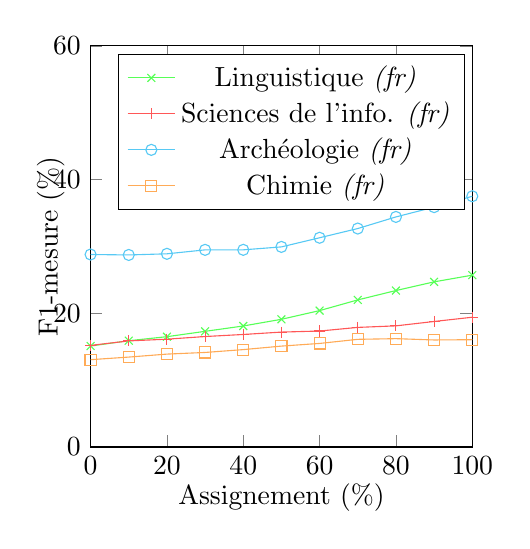
\begin{tikzpicture}
    \pgfkeys{/pgf/number format/.cd, fixed}
    \begin{axis}[x=0.0040\linewidth,
                 xtick={0, 20, ..., 100},
                 xmin=0,
                 xmax=100,
                 xlabel=Assignement (\%),
                 x label style={yshift=.34em},
                 y=0.007\linewidth,
                 ytick={0, 20, ..., 100},
                 ymin=0,
                 ymax=60,
                 ylabel=F1-mesure (\%),
                 y label style={yshift=-1.1em}]
      \addplot[green!66, mark=x] coordinates{
        (0, 15.1)
        (10, 15.9)
        (20, 16.5)
        (30, 17.3)
        (40, 18.1)
        (50, 19.1)
        (60, 20.4)
        (70, 22.0)
        (80, 23.4)
        (90, 24.7)
        (100, 25.7)
      };
      \addplot[red!66, mark=+] coordinates{
        (0, 15.1992)
        (10, 15.8659)
        (20, 16.1269)
        (30, 16.5223)
        (40, 16.8308)
        (50, 17.1875)
        (60, 17.3450)
        (70, 17.8887)
        (80, 18.1184)
        (90, 18.7733)
        (100, 19.4089)
      };
      \addplot[cyan!66, mark=o] coordinates{
        (0, 28.7887)
        (10, 28.7239)
        (20, 28.8927)
        (30, 29.4833)
        (40, 29.4880)
        (50, 29.9271)
        (60, 31.2943)
        (70, 32.6718)
        (80, 34.4101)
        (90, 35.8757)
        (100, 37.5003)
      };
      \addplot[orange!66, mark=square] coordinates{
        (0, 13.0605)
        (10, 13.4498)
        (20, 13.8944)
        (30, 14.1412)
        (40, 14.5673)
        (50, 15.0916)
        (60, 15.4902)
        (70, 16.1045)
        (80, 16.2055)
        (90, 16.0077)
        (100, 16.0506)
      };
      \legend{Linguistique \textit{(fr)}, Sciences de l'info. \textit{(fr)}, Archéologie \textit{(fr)}, Chimie \textit{(fr)}};
    \end{axis}
  \end{tikzpicture}
  \caption{Performance de TopicCoRank appliqué aux données Termith, lorsque
           le taux d'assignement varie
           \label{fig:assignment_variations_termith}}
\end{figure}

